\chapter{Referencial Teórico}

\section{Lâminas Histopatológicas}

\begin{figure}[h]
    \centering
    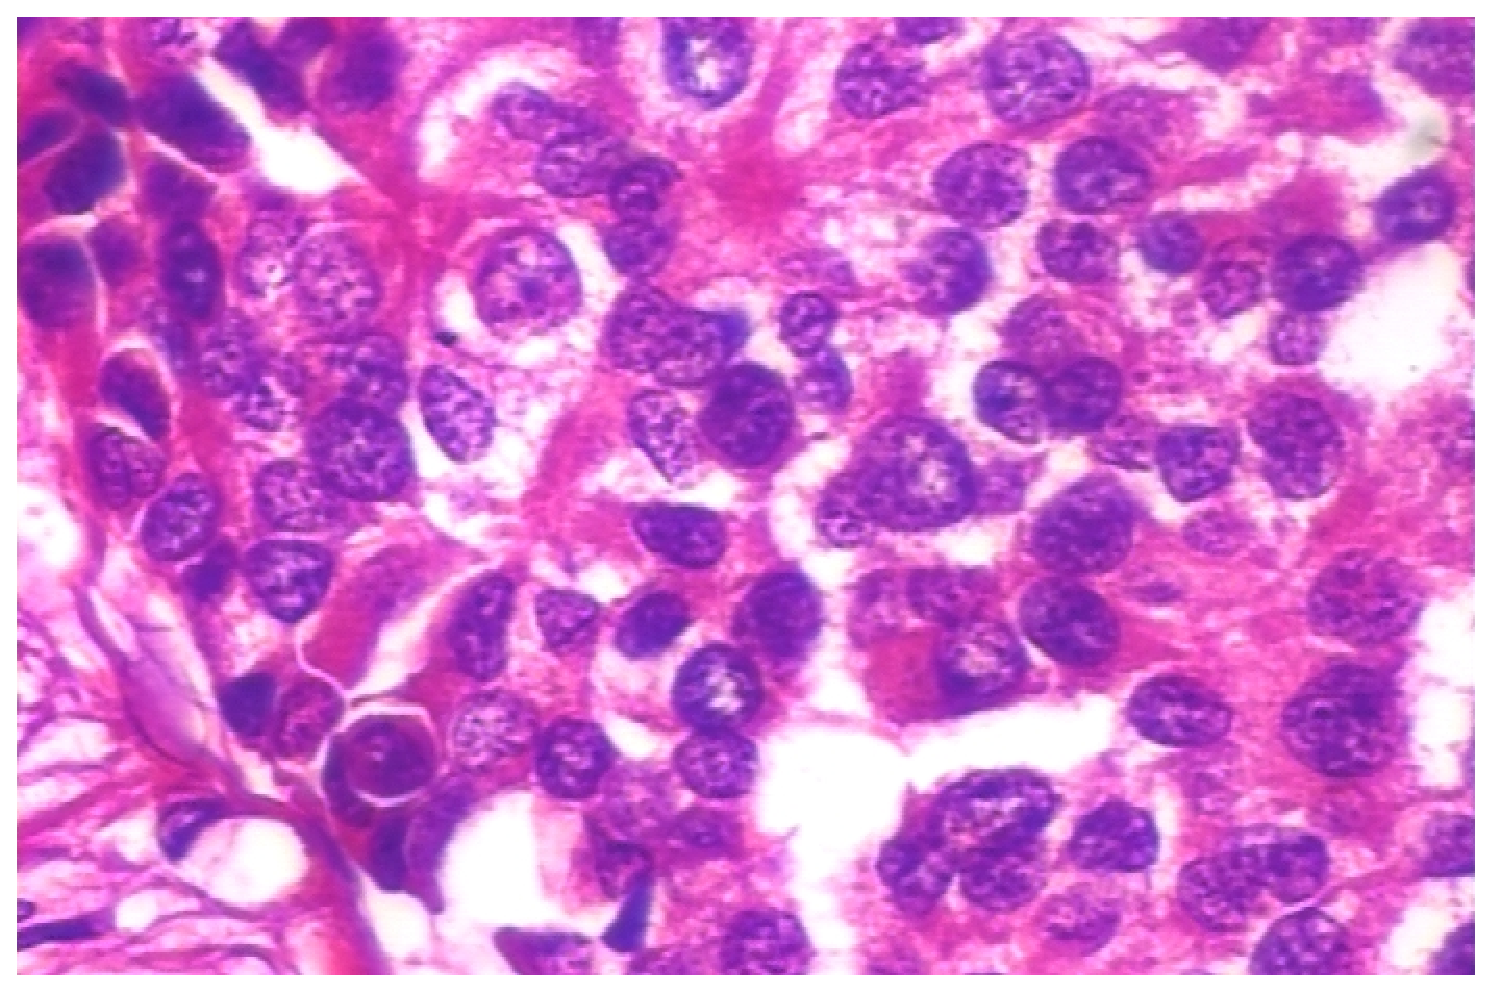
\includegraphics[width=350px, height=230px]{figuras/introducao/ductal-carcinoma-400x.eps}
    \caption{Exemplo de uma lâmina histopatológica digitalizada de um carcinoma ductal ampliada em 400x \cite{spanhol2016dataset}.}
    % \fonte{Fonte qualquer}
    \label{fig:carcinoma}
\end{figure}

\section{Patologia Computacional}

\section{Whole Slide Imaging}

\section{Processamento de Imagem}
\subsection{Detecção e Descrição de Características}
\subsection{Algoritmo SIFT}
\subsection{Algoritmo SURF}
\subsection{Algoritmo ORB}
\subsection{Características Correspondentes}
\subsection{Composição da Imagem}
\subsection{Matriz de Homografia}
\subsection{Wrap Perspective}